\documentclass[12pt, a4paper]{article}
\usepackage[T1]{fontenc}
\usepackage[utf8]{inputenc}
\usepackage{geometry}
\geometry{letterpaper}
\usepackage{graphicx}
\usepackage[danish]{babel}
\usepackage{amssymb}
\usepackage{fancyhdr}
\usepackage{amsmath,amssymb}
\usepackage{comment}
\usepackage{caption}
\usepackage{subfigure}
\usepackage{fixltx2e}
\usepackage{changepage}
\usepackage{listings}
\DeclareUnicodeCharacter{00A0}{ }
\pagestyle{fancy}

% http://tex.stackexchange.com/questions/33519/vertical-line-in-matrix-using-latexit
% Fix for bmatrix
\makeatletter
\renewcommand*\env@matrix[1][*\c@MaxMatrixCols c]{%
  \hskip -\arraycolsep
  \let\@ifnextchar\new@ifnextchar
  \array{#1}}
\makeatother

% My commands
\newcommand{\equ}[1]{\begin{align}#1\end{align}}
\newcommand{\tb}[1]{\textbf{#1}\\}
\newcommand{\tsub}[1]{\textsubscript{#1}}
\newcommand{\tsup}[1]{\textsuperscript{#1}}

\newcommand{\Lim}[1]{\raisebox{0.5ex}{\scalebox{0.8}{$\displaystyle \lim_{#1}\;$}}}

% End of my commands

\title{
  \vspace{-3em}
  {\Large \underline {Københavns Universitet}} \\
  {\Large Maskinarkitektur} \\ % Kursus
 \vspace{7em}
 \hrulefill \\
 { \huge \bfseries G2 \\[0.1cm] }
\hrulefill
}
\author{\Large {Gruppe:} \\ 
Asger Lund Hansen (CMG881) og Mads Ynddal (SJT402)\\ og Troels Ynddal (QWV828)
}

\date{
\vfill
\today
}

\rhead{\today}
\lhead{Maskinarkitektur 2014}


\begin{document}

\maketitle
\newpage


\begin{comment}
I skal skrive en rapport, hvor I kort beskriver jeres pipeline (ca. 1-2 sider).
I skal redegøre for hvilke instruktioner I har fået til at virke og eventuelle instruktioner, som I ikke har fået til at virke.
I sidste tilfælde skal I kort beskrive hvorfor I tror, at de ikke virker, og hvad man evt. kunne gøre for at få det til at virke.
Det samme gælder hazard detection og forwarding.
Sidst men ikke mindst skal jeres rapport indeholde en beskrivelse af jeres tests med forventet output og faktisk output.
\end{comment}

\section{Instruktioner}
Efter at en instruktion er blevet indlæst fra `Program Registeret', bliver instruktionens \texttt{opcode} dekodet af `Control' PLA'en. `Control' understøtter følende instruktioner:\\
\texttt{addu, addiu, slt, slti, subu, and, andi, or, ori, lw, sw, beq, jal, jr}\\

R-type instruktionerne har ikke nogen unik `opcode' (opcode'en er altid $00000$), så de bliver sendt videre, til dekodning i \texttt{EX}.
Det vil sige, at instruktionerne \texttt{addiu, slti, andi, ori, lw, sw, beq} og \texttt{jal} dekodes af `Control'. Dekodning består i at sætte de 9 kontrol-flag. De 9 flag bruges af hvert pipeline stage til at justere ALU, MUX og lignende. 

Foruden `Control' bliver instruktionen også splittet op og sendt til \texttt{rd}, register, Hazard Detection og Immediate. \texttt{rd} bruges til Hazard Detection, så den kan holde øje med hvilke registeradresser der bliver skrevet til og hvornår.

I \texttt{EX} bliver R-type instruktionerne dekodet. Da de ikke har en `opcode', skal vi dekode dem ved at læse deres `funct'. Til dette har vi lavet kredsløbet `ALUOp', som bl.a. kan læse `funct' og indstille ALU'en korrekt. Det er desuden `ALUOp', som sørger for jumps og branches bliver udregnet korrekt.

Branches bliver tjekket ved at trække to registre fra hinanden og se op ALU'ens \texttt{Zero}-flag bliver sat. Hvis de to registre ellers er ens, tjekker den, om `Branch'-flaget fra `Control' er sat. Hvis begge disse betingelser er sande, vil den aktivere en branch.


\section{Stall}
Det er lykkedes at lave et kredsløb, som kun stall'er, hvis det er nødvendigt. Det sker, hvis man ønsker at bruge \texttt{lw} efter fulgt af en instruktion, som skal bruge den indlæste værdi. I dette tilfælde, bliver der tvunget en `nop' operation ind efter \texttt{lw}. Grunden til at vi bliver nødt til at vente er, at vi normalt finder resultatet på en instruktion i \texttt{EX}, men dette glæder ikke for \texttt{lw}, da den først bliver udført i \texttt{MEM}.

\section{Hazard}

Vi har lavet vores Data Hazard ved at sammenligne instruktionen i \texttt{ID} med instruktionerne i de følgende `pipeline stages'. Hvis registeret i \texttt{ID} er ved at blive ændret på, i en anden instruktion, vil den sætte "Hazard" flaget `høj'.

Dette kan vi bruge i vores `Forwarding', til at finde frem til den nyeste instans af registeret.


\section{Forwarding}

Forwarding sker ved, at vi har en `tunnel' forbundet til slutningen af hvert `pipeline stage', så vi kan hente et resultat, som endnu ikke er blevet skrevet tilbage i registeret. Vores forwarding sker umiddelbart efter, at vi har læst fra registeret. Vi kan vha. to `mux'er', vælge om vi vil bruge værdien fra registeret, eller om vi vi forwarde en værdi fra \texttt{EX}, \texttt{MEM} eller \texttt{WB}.


\section{Branch delay slot}
Branch delay slot er supporteret ved at \texttt{beq} først bliver afgjort i \texttt{EX}-stage og derfor vil den næste instruktion nå at blive læst ind i \texttt{ID}-stage. Instruktion i \texttt{ID} bliver ikke afbrudt, fortsætter med at blive udført, hvilket giver os ét Branch delay slot.


\section{Test}





\begin{center}
\begin{tabular}{| c | c | c | }
    \hline
    	Test 1 & Test 2 & Test 3 \\ \hline
	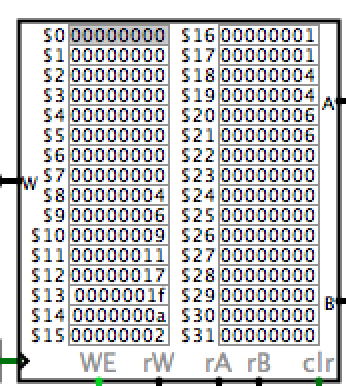
\includegraphics[width=0.15\textwidth]{1.png} &
	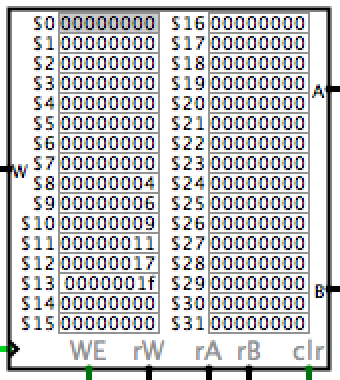
\includegraphics[width=0.15\textwidth]{r2.png}
	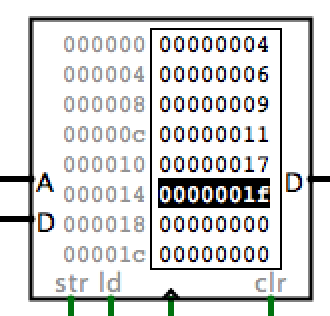
\includegraphics[width=0.15\textwidth]{2.png} & 
	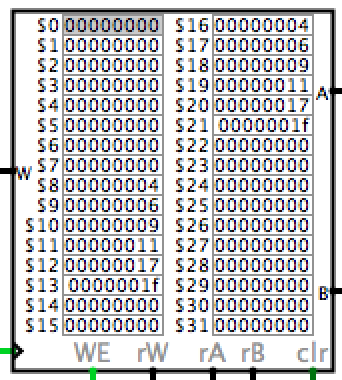
\includegraphics[width=0.15\textwidth]{3.png}
	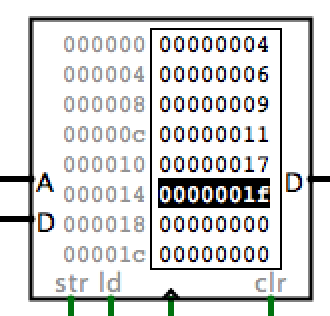
\includegraphics[width=0.15\textwidth]{2.png} \\
    \hline
\end{tabular}
\begin{tabular}{| c | c | c | c | c | }
    \hline
    	Test 4 & Test 5 & Test 6, 7 og 8 & Test 9 \\ \hline
	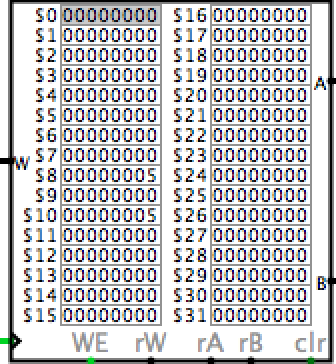
\includegraphics[width=0.15\textwidth]{4.png} &
	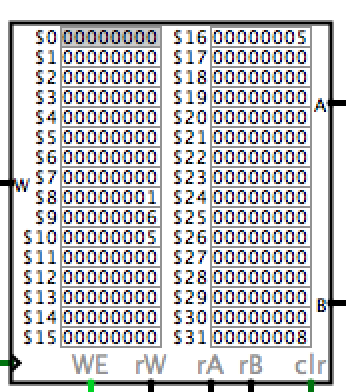
\includegraphics[width=0.15\textwidth]{5.png} &
	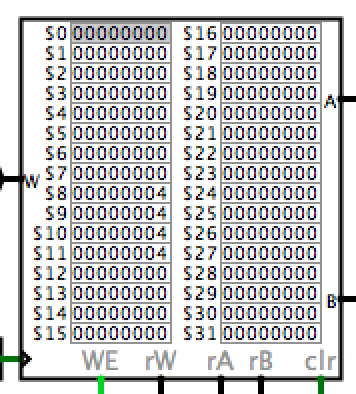
\includegraphics[width=0.15\textwidth]{6-7-8.png} &
	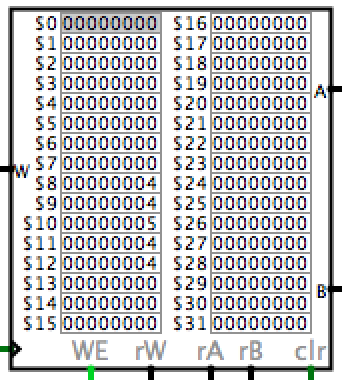
\includegraphics[width=0.15\textwidth]{9.png}
	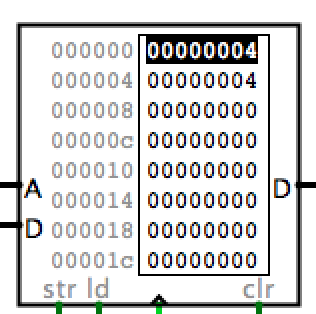
\includegraphics[width=0.15\textwidth]{s9.png}\\
    \hline
\end{tabular}

\end{center}

Vi har udført de tests der blev udleveret med opgaven. Vi har håndkørt alle testene og sammenlignet dette med resultatet fra både vores Single Cycle og Pipeline. Alle testene giver det resultat, vi havde forventet. Billederne ovenfor illustrere \textit{kun} pipeline.















\end{document}